\section{The Representative Anonymization Algorithm}
\label{sec:repOB}

We now introduce the representative anonymization algorithm (Rep-An) that combines isolated but complementary work from literature for uncertain graph anonymization. As shown in Figure\ref{fig:repOB}, we first extract a single \emph{representative} instance from an original uncertain graph. Then, conventional anonymization techniques can be then applied on this representative to attain closely approximate anonymized output of the original uncertain graph. There has been extensive work on extracting a single representative instance of uncertain graphs that capturing graph statistics such as the expected vertex degrees~\cite{Parchas_Gullo_Papadias_Bonchi_2014}. This body of research comes to its aid that anonymization can be carried out on uncertain graphs without special design for edge uncertainty.

However, the approach has several limitations. First, the input edge uncertainties (probabilities) are no longer integrated into the anonymization process since they are detached from the graph in the first phase. Second, the anonymization process (the second phase) is oblivious to the {\em reliability} metric since its input is a made-up deterministic graph. Third, since the two phases are isolated from each other, different phases are optimized for different metrics. As the result, this naive \texttt{Rep-An} approach introduces a high level of noise and consequently deteriorates the overall utility of the anonymized graph. 
In the experiment section, we further study this approach empirically and confirm its impracticality.

% Figure~\ref{fig:repOB} illustrates these limitations. The uncertain input graph (L.H.S) will have 
% the corresponding deterministic representative graph (middle) according to~\cite{Parchas_Gullo_Papadias_Bonchi_2014}. 
% This graph is viewed by the state-of-art anonymization techniques as being already anonymized and will be published as is (R.H.S top graph).
% However, it is clear that an anonymized graph with a much-higher utility can be generated, e.g., (R.H.S bottom graph).  

% % {\todo{Still References in the figure need to be fixed...}}
% % the utility loss between XXX and XXX is wrong expression 
% % {\todo{Remove the 2nd half of that Figure 3. I does not add much... And it needs more discussion on why the top part generates edges of weight 1, which does not seem to be uncertain, etc...}} 
% % {\todoB{References in the figure (on the edges) do not match the ones in text!!! Update to make them matching...}}

\begin{figure}[t]
	\vspace{-1em}
    \captionsetup{margin=0cm}
    \centering  
        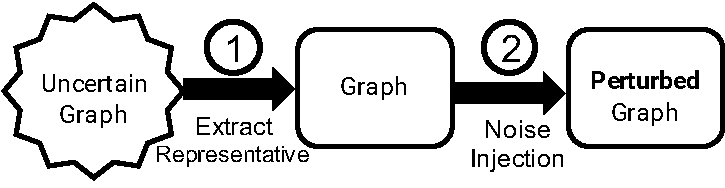
\includegraphics[width=0.95\columnwidth]{AddFigure/repOB.pdf}
        \vspace{-0.7em}
    	\caption{Overview of Rep-An. Noise is added to the extracted \emph{representative} instance.}
    \label{fig:repOB}
    \vspace{-0.5em}
\end{figure}
